% Robert Adams CS 475

\documentclass[letterpaper,10pt]{article} %twocolumn titlepage 
\usepackage{graphicx}
\usepackage{amssymb}
\usepackage{amsmath}
\usepackage{amsthm}

\usepackage{alltt}
\usepackage{float}
\usepackage{color}
\usepackage{url}

\usepackage{balance}
\usepackage[TABBOTCAP, tight]{subfigure}
\usepackage{enumitem}
\usepackage{pstricks, pst-node}


\usepackage{geometry}
\geometry{margin=0.8in, textheight=8.5in} %textwidth=6in

%random comment

\newcommand{\cred}[1]{{\color{red}#1}}
\newcommand{\cblue}[1]{{\color{blue}#1}}

\usepackage{hyperref}

\def\name{Robert Adams}
%% The following metadata will show up in the PDF properties
\hypersetup{
	colorlinks = true,
	urlcolor = black,
	pdfauthor = {\name},
	pdfkeywords = {cs745},
	pdftitle = 	{CS 475 Project 8: OpenCL Array Multiplication},
pdfsubject = {CS 475 Project 8},
	pdfpagemode = UseNone,
}


\begin{document}
\title{CS 475 Project 8: OpenCL Array Multiplication} 
\author{Robert Adams}
\maketitle



\section{Commentary}

\indent First thing to note: GPU performance absolutely destroys SIMD performance,
iny my case by a factor of over 50x. 
\\
Also of note is that modifying local work size does not affect the 
performance. I was not able to see a difference on either my home 
system (specs below), or the CGEL lab. This may be because the video
cards of both are rather out of date.  For a new, or properly setup
machine we should see performance increase as the local size increases,
since more processing power has been assigned to the task.

\subsection{System Specs}

\begin{itemize}
\item AMD Athlon II X4 630 Processor, 2800 Mhz, 4 Cores, 4 Logical Processors
\item 4.00 GB RAM
\item  NVIDIA GeForce 98000 GT, 512MB RAM
\item  Driver Version 8.17.13
\end{itemize}


\pagebreak

\begin{figure} [ht]
	\centering
	% GNUPLOT: LaTeX picture with Postscript
\begingroup
  \makeatletter
  \providecommand\color[2][]{%
    \GenericError{(gnuplot) \space\space\space\@spaces}{%
      Package color not loaded in conjunction with
      terminal option `colourtext'%
    }{See the gnuplot documentation for explanation.%
    }{Either use 'blacktext' in gnuplot or load the package
      color.sty in LaTeX.}%
    \renewcommand\color[2][]{}%
  }%
  \providecommand\includegraphics[2][]{%
    \GenericError{(gnuplot) \space\space\space\@spaces}{%
      Package graphicx or graphics not loaded%
    }{See the gnuplot documentation for explanation.%
    }{The gnuplot epslatex terminal needs graphicx.sty or graphics.sty.}%
    \renewcommand\includegraphics[2][]{}%
  }%
  \providecommand\rotatebox[2]{#2}%
  \@ifundefined{ifGPcolor}{%
    \newif\ifGPcolor
    \GPcolorfalse
  }{}%
  \@ifundefined{ifGPblacktext}{%
    \newif\ifGPblacktext
    \GPblacktexttrue
  }{}%
  % define a \g@addto@macro without @ in the name:
  \let\gplgaddtomacro\g@addto@macro
  % define empty templates for all commands taking text:
  \gdef\gplbacktext{}%
  \gdef\gplfronttext{}%
  \makeatother
  \ifGPblacktext
    % no textcolor at all
    \def\colorrgb#1{}%
    \def\colorgray#1{}%
  \else
    % gray or color?
    \ifGPcolor
      \def\colorrgb#1{\color[rgb]{#1}}%
      \def\colorgray#1{\color[gray]{#1}}%
      \expandafter\def\csname LTw\endcsname{\color{white}}%
      \expandafter\def\csname LTb\endcsname{\color{black}}%
      \expandafter\def\csname LTa\endcsname{\color{black}}%
      \expandafter\def\csname LT0\endcsname{\color[rgb]{1,0,0}}%
      \expandafter\def\csname LT1\endcsname{\color[rgb]{0,1,0}}%
      \expandafter\def\csname LT2\endcsname{\color[rgb]{0,0,1}}%
      \expandafter\def\csname LT3\endcsname{\color[rgb]{1,0,1}}%
      \expandafter\def\csname LT4\endcsname{\color[rgb]{0,1,1}}%
      \expandafter\def\csname LT5\endcsname{\color[rgb]{1,1,0}}%
      \expandafter\def\csname LT6\endcsname{\color[rgb]{0,0,0}}%
      \expandafter\def\csname LT7\endcsname{\color[rgb]{1,0.3,0}}%
      \expandafter\def\csname LT8\endcsname{\color[rgb]{0.5,0.5,0.5}}%
    \else
      % gray
      \def\colorrgb#1{\color{black}}%
      \def\colorgray#1{\color[gray]{#1}}%
      \expandafter\def\csname LTw\endcsname{\color{white}}%
      \expandafter\def\csname LTb\endcsname{\color{black}}%
      \expandafter\def\csname LTa\endcsname{\color{black}}%
      \expandafter\def\csname LT0\endcsname{\color{black}}%
      \expandafter\def\csname LT1\endcsname{\color{black}}%
      \expandafter\def\csname LT2\endcsname{\color{black}}%
      \expandafter\def\csname LT3\endcsname{\color{black}}%
      \expandafter\def\csname LT4\endcsname{\color{black}}%
      \expandafter\def\csname LT5\endcsname{\color{black}}%
      \expandafter\def\csname LT6\endcsname{\color{black}}%
      \expandafter\def\csname LT7\endcsname{\color{black}}%
      \expandafter\def\csname LT8\endcsname{\color{black}}%
    \fi
  \fi
  \setlength{\unitlength}{0.0500bp}%
  \begin{picture}(9792.00,5040.00)%
    \gplgaddtomacro\gplbacktext{%
      \csname LTb\endcsname%
      \put(1210,744){\makebox(0,0)[r]{\strut{} 0}}%
      \put(1210,1551){\makebox(0,0)[r]{\strut{} 100}}%
      \put(1210,2357){\makebox(0,0)[r]{\strut{} 200}}%
      \put(1210,3163){\makebox(0,0)[r]{\strut{} 300}}%
      \put(1210,3970){\makebox(0,0)[r]{\strut{} 400}}%
      \put(1210,4776){\makebox(0,0)[r]{\strut{} 500}}%
      \put(1342,484){\makebox(0,0){\strut{} 0}}%
      \put(2465,484){\makebox(0,0){\strut{} 500000}}%
      \put(3588,484){\makebox(0,0){\strut{} 1e+06}}%
      \put(4711,484){\makebox(0,0){\strut{} 1.5e+06}}%
      \put(5833,484){\makebox(0,0){\strut{} 2e+06}}%
      \put(6956,484){\makebox(0,0){\strut{} 2.5e+06}}%
      \put(8079,484){\makebox(0,0){\strut{} 3e+06}}%
      \put(440,2740){\rotatebox{90}{\makebox(0,0){\strut{}GFLOPS/sec}}}%
      \put(4710,154){\makebox(0,0){\strut{}Global Size}}%
    }%
    \gplgaddtomacro\gplfronttext{%
      \csname LTb\endcsname%
      \put(8805,4666){\makebox(0,0)[r]{\strut{}1}}%
      \csname LTb\endcsname%
      \put(8805,4446){\makebox(0,0)[r]{\strut{}2}}%
      \csname LTb\endcsname%
      \put(8805,4226){\makebox(0,0)[r]{\strut{}4}}%
      \csname LTb\endcsname%
      \put(8805,4006){\makebox(0,0)[r]{\strut{}8}}%
      \csname LTb\endcsname%
      \put(8805,3786){\makebox(0,0)[r]{\strut{}16}}%
      \csname LTb\endcsname%
      \put(8805,3566){\makebox(0,0)[r]{\strut{}32}}%
      \csname LTb\endcsname%
      \put(8805,3346){\makebox(0,0)[r]{\strut{}64}}%
      \csname LTb\endcsname%
      \put(8805,3126){\makebox(0,0)[r]{\strut{}128}}%
      \csname LTb\endcsname%
      \put(8805,2906){\makebox(0,0)[r]{\strut{}256}}%
      \csname LTb\endcsname%
      \put(8805,2686){\makebox(0,0)[r]{\strut{}512}}%
      \csname LTb\endcsname%
      \put(8805,2466){\makebox(0,0)[r]{\strut{}1024}}%
      \csname LTb\endcsname%
      \put(8805,2246){\makebox(0,0)[r]{\strut{}SIMD}}%
    }%
    \gplbacktext
    \put(0,0){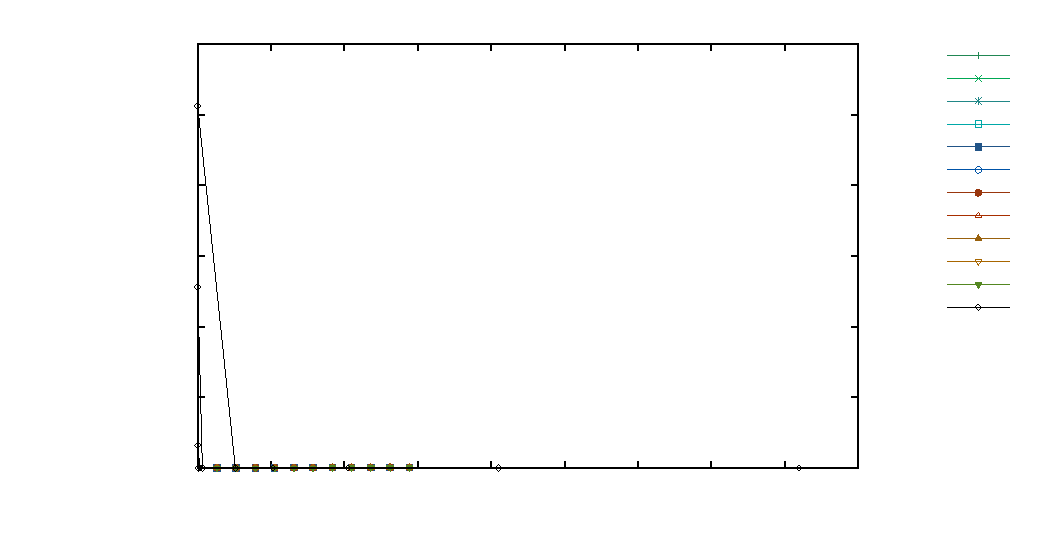
\includegraphics{global}}%
    \gplfronttext
  \end{picture}%
\endgroup

	%\caption{Speed of height calculations performed on a subdivided surface} 
	\label{runtimes}
\end{figure}

\begin{figure} [ht]
	\centering
	% GNUPLOT: LaTeX picture with Postscript
\begingroup
  \makeatletter
  \providecommand\color[2][]{%
    \GenericError{(gnuplot) \space\space\space\@spaces}{%
      Package color not loaded in conjunction with
      terminal option `colourtext'%
    }{See the gnuplot documentation for explanation.%
    }{Either use 'blacktext' in gnuplot or load the package
      color.sty in LaTeX.}%
    \renewcommand\color[2][]{}%
  }%
  \providecommand\includegraphics[2][]{%
    \GenericError{(gnuplot) \space\space\space\@spaces}{%
      Package graphicx or graphics not loaded%
    }{See the gnuplot documentation for explanation.%
    }{The gnuplot epslatex terminal needs graphicx.sty or graphics.sty.}%
    \renewcommand\includegraphics[2][]{}%
  }%
  \providecommand\rotatebox[2]{#2}%
  \@ifundefined{ifGPcolor}{%
    \newif\ifGPcolor
    \GPcolorfalse
  }{}%
  \@ifundefined{ifGPblacktext}{%
    \newif\ifGPblacktext
    \GPblacktexttrue
  }{}%
  % define a \g@addto@macro without @ in the name:
  \let\gplgaddtomacro\g@addto@macro
  % define empty templates for all commands taking text:
  \gdef\gplbacktext{}%
  \gdef\gplfronttext{}%
  \makeatother
  \ifGPblacktext
    % no textcolor at all
    \def\colorrgb#1{}%
    \def\colorgray#1{}%
  \else
    % gray or color?
    \ifGPcolor
      \def\colorrgb#1{\color[rgb]{#1}}%
      \def\colorgray#1{\color[gray]{#1}}%
      \expandafter\def\csname LTw\endcsname{\color{white}}%
      \expandafter\def\csname LTb\endcsname{\color{black}}%
      \expandafter\def\csname LTa\endcsname{\color{black}}%
      \expandafter\def\csname LT0\endcsname{\color[rgb]{1,0,0}}%
      \expandafter\def\csname LT1\endcsname{\color[rgb]{0,1,0}}%
      \expandafter\def\csname LT2\endcsname{\color[rgb]{0,0,1}}%
      \expandafter\def\csname LT3\endcsname{\color[rgb]{1,0,1}}%
      \expandafter\def\csname LT4\endcsname{\color[rgb]{0,1,1}}%
      \expandafter\def\csname LT5\endcsname{\color[rgb]{1,1,0}}%
      \expandafter\def\csname LT6\endcsname{\color[rgb]{0,0,0}}%
      \expandafter\def\csname LT7\endcsname{\color[rgb]{1,0.3,0}}%
      \expandafter\def\csname LT8\endcsname{\color[rgb]{0.5,0.5,0.5}}%
    \else
      % gray
      \def\colorrgb#1{\color{black}}%
      \def\colorgray#1{\color[gray]{#1}}%
      \expandafter\def\csname LTw\endcsname{\color{white}}%
      \expandafter\def\csname LTb\endcsname{\color{black}}%
      \expandafter\def\csname LTa\endcsname{\color{black}}%
      \expandafter\def\csname LT0\endcsname{\color{black}}%
      \expandafter\def\csname LT1\endcsname{\color{black}}%
      \expandafter\def\csname LT2\endcsname{\color{black}}%
      \expandafter\def\csname LT3\endcsname{\color{black}}%
      \expandafter\def\csname LT4\endcsname{\color{black}}%
      \expandafter\def\csname LT5\endcsname{\color{black}}%
      \expandafter\def\csname LT6\endcsname{\color{black}}%
      \expandafter\def\csname LT7\endcsname{\color{black}}%
      \expandafter\def\csname LT8\endcsname{\color{black}}%
    \fi
  \fi
  \setlength{\unitlength}{0.0500bp}%
  \begin{picture}(9792.00,5040.00)%
    \gplgaddtomacro\gplbacktext{%
      \csname LTb\endcsname%
      \put(990,704){\makebox(0,0)[r]{\strut{} 0}}%
      \put(990,1111){\makebox(0,0)[r]{\strut{} 50}}%
      \put(990,1518){\makebox(0,0)[r]{\strut{} 100}}%
      \put(990,1926){\makebox(0,0)[r]{\strut{} 150}}%
      \put(990,2333){\makebox(0,0)[r]{\strut{} 200}}%
      \put(990,2740){\makebox(0,0)[r]{\strut{} 250}}%
      \put(990,3147){\makebox(0,0)[r]{\strut{} 300}}%
      \put(990,3554){\makebox(0,0)[r]{\strut{} 350}}%
      \put(990,3962){\makebox(0,0)[r]{\strut{} 400}}%
      \put(990,4369){\makebox(0,0)[r]{\strut{} 450}}%
      \put(990,4776){\makebox(0,0)[r]{\strut{} 500}}%
      \put(1122,484){\makebox(0,0){\strut{} 0}}%
      \put(2216,484){\makebox(0,0){\strut{} 200}}%
      \put(3309,484){\makebox(0,0){\strut{} 400}}%
      \put(4403,484){\makebox(0,0){\strut{} 600}}%
      \put(5496,484){\makebox(0,0){\strut{} 800}}%
      \put(6590,484){\makebox(0,0){\strut{} 1000}}%
      \put(7683,484){\makebox(0,0){\strut{} 1200}}%
      \put(4402,154){\makebox(0,0){\strut{}Local Size}}%
    }%
    \gplgaddtomacro\gplfronttext{%
      \csname LTb\endcsname%
      \put(8805,4666){\makebox(0,0)[r]{\strut{}262144}}%
      \csname LTb\endcsname%
      \put(8805,4446){\makebox(0,0)[r]{\strut{}524288}}%
      \csname LTb\endcsname%
      \put(8805,4226){\makebox(0,0)[r]{\strut{}786432}}%
      \csname LTb\endcsname%
      \put(8805,4006){\makebox(0,0)[r]{\strut{}1048576}}%
      \csname LTb\endcsname%
      \put(8805,3786){\makebox(0,0)[r]{\strut{}1310720}}%
      \csname LTb\endcsname%
      \put(8805,3566){\makebox(0,0)[r]{\strut{}1572864}}%
      \csname LTb\endcsname%
      \put(8805,3346){\makebox(0,0)[r]{\strut{}1835008}}%
      \csname LTb\endcsname%
      \put(8805,3126){\makebox(0,0)[r]{\strut{}2097152}}%
      \csname LTb\endcsname%
      \put(8805,2906){\makebox(0,0)[r]{\strut{}2359296}}%
      \csname LTb\endcsname%
      \put(8805,2686){\makebox(0,0)[r]{\strut{}2621440}}%
      \csname LTb\endcsname%
      \put(8805,2466){\makebox(0,0)[r]{\strut{}2883584}}%
    }%
    \gplbacktext
    \put(0,0){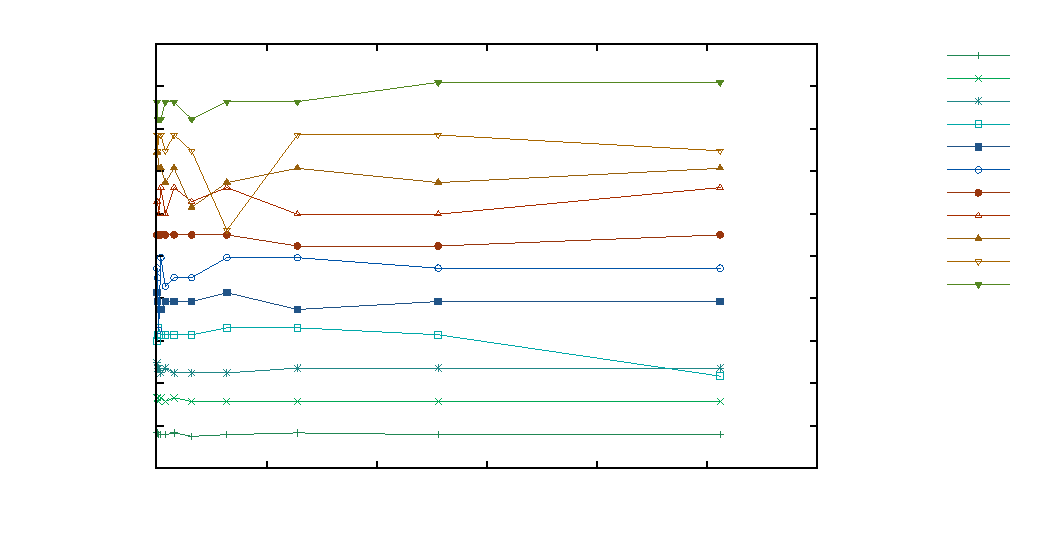
\includegraphics{local}}%
    \gplfronttext
  \end{picture}%
\endgroup

	%\caption{Speed of height calculations performed on a subdivided surface} 
	\label{runtimes}
\end{figure}

%\begin{table}  [ht]
	%\centering
	%    \begin{tabular}{llllll}
%\verb|#|months & precipitation, in. & temperature, celsuis & height, in.
               %& \#deer & blood rain\\ \hline 
%0 & 7.130446 & 3.047354 & 7.280658 & 1 & 0\\ 
%1 & 11.88923 & 5.459258 & 7.399446 & 2 & 0\\ 
%2 & 12.868473 & 5.293376 & 7.097805 & 3 & 0\\ 
%3 & 11.705143 & 13.475433 & 0 & 4 & 0\\ 

		%    \end{tabular}
	%\end{table}

	\end{document}
